% !TeX program = pdflatex
\documentclass[russian,utf8,simple]{eskdtext}

% packages
%
% Тестовое наполнение текстом
% При написании работы - удалить пакет и комманды \lipsum
\usepackage{lipsum}
%
\usepackage{graphicx}
\usepackage{datetime}
\usepackage{enumitem} % for lists
\usepackage{ulem} % for underlining
\usepackage{lastpage} % Number of pages
\usepackage{hyperref} % Links in pdf

% setup
\newcommand{\FrontPageDepartment}{ИТ} %Факультет
\newcommand{\FrontPageSubdepartment}{САПР} %Кафедра
\newcommand{\WorkType}{Лабораторная работа №3} %Тип работы (заголовок)
\newcommand{\Subject}{Инструментальные средства разработки программного обеспечения} %по ... родительный падеж
\newcommand{\Topic}{Разработка приложения на языке C\# с использованием WPF} %Тема
\newcommand{\Professor}{Пугин~Е.~В.} %Руководитель
\newcommand{\Student}{Шипин~Е.~С.} %Студент
\newcommand{\Group}{ПКС-216} %Группа
\newcommand{\FrontPageDate}{\ddmmyyyydate\today} %Дата

\ESKDsignature{МИВУ 090203.68 ПЗ} % Код специальности и тип работы

% eskdx setup
\ESKDletter{}{У}{}
\ESKDtitle{\Topic}
\ESKDchecker{\Professor}
\ESKDauthor{\Student}
\ESKDcolumnIX{МИ ВлГУ\\ \Group}

\addto\captionsrussian{\def\refname{Список использованных источников}}
\sloppy % split long lines

% graphics path
\graphicspath{{src/img/}}


% verbatim setup
\newcommand{\verbatimFont}{
\fontsize{10pt}{12pt}\selectfont
\baselineskip=1em
}


% workaround for regression in babel package on linux
\providecommand{\No}{\textnumero}


% remove vertical space from lists
%\renewcommand{\alph}[1]{\asbuk{#1}} % костыль для кирилической нумерации вместо латинской
\setlist{nolistsep} % убираем дополнительные вертикальные отступы вокруг списков
\setenumerate[1]{label=\arabic*), fullwidth, itemindent=\parindent,  listparindent=\parindent}
\setenumerate[2]{label=\arabic*), fullwidth, itemindent=\parindent, listparindent=\parindent, leftmargin=\parindent}
\setitemize{fullwidth, itemindent=\parindent, listparindent=\parindent}

% main document
\begin{document}
% Титул
\ESKDthisStyle{title}
\newlength{\frontpagefk} % Ширина поля Факультет/Кафедра
\setlength{\frontpagefk}{6cm}
\newlength{\frontpagerb} % Ширина надписей Руководитель/Студент и пр. под темой
\setlength{\frontpagerb}{6cm}
\newlength{\frontpagerbspace} % ??? (do not remove)
\setlength{\frontpagerbspace}{1cm}
\newlength{\FrontPageSubjSpace} % Ширина пробела до и после названия предмета
\setlength{\FrontPageSubjSpace}{1cm}
\newlength{\FrontPageTopicSpace} % Ширина пробела до и после темы
\setlength{\FrontPageTopicSpace}{0.5cm}

\thispagestyle{empty}
\begin{center}
{
\vspace*{-1.5cm}
\baselineskip=1.3em
{\small Министерство образования и науки Российской Федерации}\\
\textbf{Муромский институт (филиал)}\\
{\footnotesize федерального государственного бюджетного образовательного учреждения\\
высшего профессионального образования}\\
\textbf{<<Владимирский государственный университет\\
имени Александра Григорьевича и Николая Григорьевича\\
Столетовых>>\\
(МИВлГУ)\\}
}

\bigskip
\begin{tabular}{l c}
\textbf{Факультет}&\underline{\makebox[\frontpagefk]{\FrontPageDepartment}}\\
\textbf{Кафедра}&\underline{\makebox[\frontpagefk]{\FrontPageSubdepartment}}\\
\end{tabular}

\vspace{\fill}
\begin{Huge}
\textbf{\textsl{\WorkType}}
\end{Huge}

\vspace{\fill}
по \underline{\makebox[\FrontPageSubjSpace]{}\Subject\makebox[\FrontPageSubjSpace]{}}

\smallskip
\parbox{15cm}{\centering{Тема: \uline{\makebox[\FrontPageTopicSpace]{}\Topic\makebox[\FrontPageTopicSpace]{}}}}

\vspace{\fill}

\begin{flushright}
\makebox[\frontpagerb][c]{
\makebox[\frontpagerb][l]{Руководитель}\hspace{\frontpagerbspace}}

\smallskip
\makebox[\frontpagerb][c]{
\raisebox{-\baselineskip}{\shortstack{\underline{\makebox[\frontpagerb][l]{\Professor}}\\
\begin{footnotesize}
(фамилия, инициалы)
\end{footnotesize}}}\hspace{\frontpagerbspace}}

\bigskip
\makebox[\frontpagerb][c]{
\raisebox{-\baselineskip}{\shortstack{\underline{\makebox[\frontpagerb][l]{}}\\
\begin{footnotesize}
(подпись)\hfill(дата)
\end{footnotesize}}}\hspace{\frontpagerbspace}}

\newcommand{\frontpagerbstudent}[2]{ %
\makebox[\frontpagerb]{ %
\raisebox{-\baselineskip}{\shortstack{#1\ \underline{\makebox[\frontpagerb-\widthof{#1\ }][c]{#2}}\\
\begin{footnotesize}
\makebox[\widthof{#1\ }][c]{}\makebox[\frontpagerb-\widthof{#1\ }][c]{(группа)}
\end{footnotesize}}}\hspace{\frontpagerbspace}}
}

\bigskip
\makebox[\frontpagerb][c]{\frontpagerbstudent{Студент}{\Group}}

\smallskip
\makebox[\frontpagerb][c]{
\raisebox{-\baselineskip}{\shortstack{\underline{\makebox[\frontpagerb][l]{\Student}}\\
\begin{footnotesize}
(фамилия, инициалы)
\end{footnotesize}}}\hspace{\frontpagerbspace}}

\renewcommand{\dateseparator}{.}

\bigskip
\makebox[\frontpagerb][c]{
\raisebox{-\baselineskip}{\shortstack{\underline{\makebox[\frontpagerb][r]{\FrontPageDate}}\\
\begin{footnotesize}
(подпись)\hfill(дата)
\end{footnotesize}}}\hspace{\frontpagerbspace}}

\end{flushright}

\vspace{\fill}
Муром \the\year
\vspace*{-1cm}
\end{center}
\newpage

% Основной текст
\ESKDthisStyle{formII}  %2 страница рамки

\begin{center}
\textbf{Лабораторная работа №3}
\\
\textbf{Тема:} Разработка приложения на языке C\# с использованием WPF.
\\
Цель:В ходе лабораторной работы необходимо научится разрабатывать программы с использованием WPF.  
\end{center}

Задание:
\begin{enumerate}

\item В Visual Studio 2017 создать проект C\# “Приложение WPF”.\
\item Добавить в проект компонент “WPF компонент (виджет)”.
\item Разработать на этом компоненте программу калькулятор.
\item Добавить компонент на главную форму, проверить работоспособность программы.

\end{enumerate}

Код программы:

using System;\\
using System.Collections.Generic;\\
using System.Linq;\\
using System.Text;\\
using System.Threading.Tasks;\\
using System.Windows;\\
using System.Windows.Controls;\\
using System.Windows.Data;\\
using System.Windows.Documents;\\
using System.Windows.Input;\\
using System.Windows.Media;\\
using System.Windows.Media.Imaging;\\
using System.Windows.Navigation;\\
using System.Windows.Shapes;\\

namespace WpfApp1\\
\{\\
    /// <summary>\\
    /// Логика взаимодействия для MainWindow.xaml\\
    /// </summary>\\
    public partial class MainWindow : Window\\
    \{\\
        public MainWindow()\\
        \{\\
            InitializeComponent();\\
        \}\\

        public double c = 0;\\
        bool plus1 = false;\\
        bool minus1 = false;\\
        bool umnoj1 = false;\\
        bool delenie1 = false;\\
        bool point1 = false;\\

        private void Button\_Click(object sender, RoutedEventArgs e)\\
        \{\\
            texb.Text += 0;\\
        \}\\

        private void one\_Click(object sender, RoutedEventArgs e)\\
        \{\\
            texb.Text += 1;\\
        \}\\

        private void two\_Click(object sender, RoutedEventArgs e)\\
        \{\\
            texb.Text += 2;\\
        \}\\

        private void three\_Click(object sender, RoutedEventArgs e)\\
        \{\\
            texb.Text += 3;\\
        \}\\

        private void four\_Click(object sender, RoutedEventArgs e)\\
        \{\\
            texb.Text += 4;\\
        \}\\

        private void five\_Click(object sender, RoutedEventArgs e)\\
        \{\\
            texb.Text += 5;\\
        \}\\

        private void six\_Click(object sender, RoutedEventArgs e)\\
        \{\\
            texb.Text += 6;\\
        \}\\

        private void seven\_Click(object sender, RoutedEventArgs e)\\
        \{\\
            texb.Text += 7;\\
        \}\\

        private void eight\_Click(object sender, RoutedEventArgs e)\\
        \{\\
            texb.Text += 8;\\
        \}\\

        private void nine\_Click(object sender, RoutedEventArgs e)\\
        \{\\
            texb.Text += 9;\\
        \}\\

        private void point\_Click(object sender, RoutedEventArgs e)\\
        \{\\
            texb.Text += ',';\\
            point.IsEnabled = false;\\
        \}\\

        private void C\_Click(object sender, RoutedEventArgs e)\\
        \{\\
            if (texb.Text.Length != 0) \\
            texb.Text = texb.Text.Substring(0, texb.Text.Length - 1);\\
            for (int i = 0; i < texb.Text.Length; i++)\\
                if (texb.Text[i] == ',')\\
                \{\\
                    point1 = true;\\
                    break;\\
                \}\\
            if (point1 == true)\\
                point.IsEnabled = false;\\

            else\\
                point.IsEnabled = true;\\


        \}\\

        private void CE\_Click(object sender, RoutedEventArgs e)\\
        \{\\
            texb.Text = "";\\
        \}\\

        private void delenie\_Click(object sender, RoutedEventArgs e)\\
        \{\\
            delenie1 = true;\\
            c = Convert.ToDouble(texb.Text);\\
            texb.Text = "";\\
        \}\\

        private void umnojenie\_Click(object sender, RoutedEventArgs e)\\
        \{\\
            umnoj1 = true;\\
            c = Convert.ToDouble(texb.Text);\\
            texb.Text = "";\\
        \}\\

        private void minus\_Click(object sender, RoutedEventArgs e)\\
        \{\\
            minus1 = true;\\
            c = Convert.ToDouble(texb.Text);\\
            texb.Text = "";\\
        \}\\

        private void ravno\_Click(object sender, RoutedEventArgs e)\\
        \{\\
            if (plus1 == true)\\
            \{\\
                c += Convert.ToDouble(texb.Text);\\
                plus1 = false;
            \}\\

            else\\
            if (minus1 == true)\\
            \{\\
                c -= Convert.ToDouble(texb.Text);\\
                minus1 = false;\\
            \}\\

            else\\
            if (umnoj1 == true)\\
            \{\\
                c *= Convert.ToDouble(texb.Text);\\
                umnoj1 = false;\\
            \}\\

            else\\
            if (delenie1 == true)\\
            \{\\
                c /= Convert.ToDouble(texb.Text);\\
                delenie1 = false;\\
            \}\\

            else\\
                c = Convert.ToDouble(texb.Text);\\

            texb.Text = Convert.ToString(c);\\              
        \}\\

        private void plus\_Click(object sender, RoutedEventArgs e)\\
        \{\\
            plus1 = true;\\
            c = Convert.ToDouble(texb.Text);\\
            texb.Text = "";\\

        \}\\
    \}\\
\}\\


XAML Код:
\begin{verbatim}
<Window x:Class="WpfApp1.MainWindow"
        xmlns="http://schemas.microsoft.com/winfx/2006/xaml
/presentation"
        xmlns:x="http://schemas.microsoft.com/winfx/2006/xaml"
        xmlns:d="http://schemas.microsoft.com/expression/blend/2008"
        xmlns:mc="http://schemas.openxmlformats.org/markup-
compatibility/2006"
        xmlns:local="clr-namespace:WpfApp1"
        mc:Ignorable="d"
        Title="Калькулятор" Height="567.028" Width="770.128">
    <Grid Margin="-36,0,-8,-21">
        <Grid.RowDefinitions>

        </Grid.RowDefinitions>
        <Grid.ColumnDefinitions>



        </Grid.ColumnDefinitions>\\
        <TextBox x:Name="texb" HorizontalAlignment="Stretch"
 Height="44" Margin="74,10,221,0" TextWrapping="Wrap"
 VerticalAlignment="Top" FontSize="18" IsEnabled="False"/>
        <Button x:Name="two" Content="2" Margin="331,176,359,0"
 VerticalAlignment="Top" Height="54" Click="two\_Click"/>
        <Button x:Name="three" Content="3" HorizontalAlignment=
"Left" Margin="469,176,0,327" Width="106" Click="three\_Click" 
RenderTransformOrigin="1.812,0.294"/>
        <Button x:Name="minus" Content="\-" HorizontalAlignment=
"Left" Margin="74,411,0,0" VerticalAlignment="Top" 
Width="106" Height="54" Click="minus\_Click" IsEnabled=
"{Binding ElementName=texb, Path=Text.Length}" />
        <Button x:Name="four" Content="4" HorizontalAlignment=
"Left" Margin="77,255,0,0" VerticalAlignment="Top" Width="99" 
Height="54" Click="four\_Click" RenderTransformOrigin="-0.456,0.794">
            <Button.RenderTransform>
                <TransformGroup>
                    <ScaleTransform/>
                    <SkewTransform AngleY="-1.195"/>
                    <RotateTransform Angle="0.756"/>
                    <TranslateTransform Y="1.974"/>
                </TransformGroup>
            </Button.RenderTransform>
        </Button>\\
        <Button x:Name="five" Content="5" HorizontalAlignment=
"Left" Margin="202,255,0,0" VerticalAlignment="Top" Width="106"
 Height="54" Click="five\_Click" RenderTransformOrigin="-0.427,0.191"/>
        <Button x:Name="six" Content="6" HorizontalAlignment=
"Left" Margin="331,255,0,0" VerticalAlignment="Top"
 Width="106" Height="54" Click="six\_Click"/>
        <Button x:Name="umnojenie" Content="*" HorizontalAlignment
="Left" Margin="202,411,0,0" VerticalAlignment="Top" Width=
"106" Height="54" Click="umnojenie\_Click" IsEnabled=
"{Binding ElementName=texb, Path=Text.Length}"
 RenderTransformOrigin="0.92,2.435" />
        <Button x:Name="seven" Content="7" HorizontalAlignment
="Left" VerticalAlignment="Top" Width="108" Height="54"
 Click="seven\_Click" Margin="469,255,0,0" RenderTransformOrigin
="6.394,-2.179"/>
        <Button x:Name="eight" Content="8" HorizontalAlignment
="Left" Margin="74,338,0,0" VerticalAlignment="Top" Width="106"
 Height="54" Click="eight\_Click" RenderTransformOrigin="0.24,1.581"/>
        <Button x:Name="nine" Content="9" HorizontalAlignment
="Left" Margin="202,338,0,0" VerticalAlignment="Top" Width=
"106" Height="54" Click="nine\_Click"/>
        <Button x:Name="delenie" Content="/" HorizontalAlignment
="Left" Margin="331,411,0,0" VerticalAlignment="Top" Width="106"
 Height="54" Click="delenie\_Click" IsEnabled="{Binding ElementName=
        <Button x:Name="one" Content="1" HorizontalAlignment
="Left" Margin="202,176,0,0" VerticalAlignment="Top"
 Width="106" Height="54" Click="one\_Click" RenderTransformOrigin
="4.092,3.108"/>
        <Button Content="0" HorizontalAlignment="Left"
 Margin="74,176,0,327" Width="106" Click="Button\_Click"
 RenderTransformOrigin="0.276,-2.646"/>
        <Button x:Name="point" Content="," HorizontalAlignment=
"Left" Margin="331,338,0,0" VerticalAlignment="Top" 
Width="106" Height="54" Click="poin\_Click" IsEnabled=
"{Binding ElementName=texb, Path=Text.Length}"    />
        <Button x:Name="plus" Content="+" HorizontalAlignment="
Left" Margin="469,338,0,0" VerticalAlignment="Top" Width="106" 
Height="54" Click="plus\_Click" IsEnabled="{Binding ElementName=texb,
 Path=Text.Length}" RenderTransformOrigin="-0.538,0.668" />
        <Button x:Name="ravno" Content="=" HorizontalAlignment
="Left" Margin="469,411,0,0" VerticalAlignment="Top" Width=
"108" Height="54" RenderTransformOrigin="0.234,0.67" Click=
"ravno\_Click" IsEnabled="{Binding ElementName=texb, 
Path=Text.Length}" />
        <Button x:Name="CE" Content="CE" HorizontalAlignment=
"Left" Margin="331,100,0,0" VerticalAlignment="Top" Width="244"
 Height="58" Click="CE\_Click" IsEnabled="{Binding ElementName=texb,
 Path=Text.Length}" />
        <Button x:Name="C" Content="C" HorizontalAlignment=
"Left" Margin="74,100,0,0" VerticalAlignment="Top" Width="234"
 Height="58" Click="C\_Click" IsEnabled="{Binding ElementName=texb,
 Path=Text.Length}" />

    </Grid>
</Window>
\end{verbatim}





\begin{figure}[h]% добавляем рисунок.
\centering
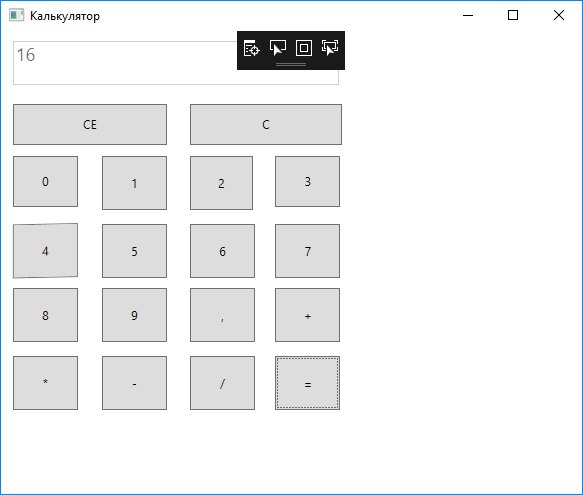
\includegraphics[scale=0.6]{Plus}
\caption{выполнение операции сложение}
\label{fig:Plus}
\end{figure}




\newpage
\textbf{Вывод:}
В ходе лабораторной работы я научился разрабатывать программы  с использованием WPF.





\newpage

\end{document}